 
\documentclass[showpacs,showkeys,preprint,prd,nofootinbib,linenumbers,12pt]{revtex4-1}

\usepackage{graphicx} % This is already loaded by the atlasnote class
% Just use it to include your plots!

\usepackage{rotating}
\usepackage{amsmath}
% use less space for subfigures
\usepackage{epstopdf}
\usepackage{multirow}
\usepackage{xspace}
\usepackage{rotating}
\usepackage{longtable}
\usepackage{multirow}
\usepackage{cancel}


\usepackage[breaklinks=true]{hyperref}
\hypersetup{
  colorlinks=true,
  linkcolor=blue,
  citecolor=blue,
  urlcolor=blue
}

\makeatletter
\renewcommand*\env@matrix[1][*\c@MaxMatrixCols c]{%
  \hskip -\arraycolsep
  \let\@ifnextchar\new@ifnextchar
  \array{#1}}
\makeatother



\graphicspath{{./fig/}}
\usepackage{array,tabularx,epsfig,mathrsfs,graphicx,rotating}
\usepackage{ifthen}
\usepackage{amsfonts}

\usepackage{subfigure}

\subfigcapskip = -0.7cm

\newcommand{\beq}{\begin{equation}}
  \newcommand{\eeq}{\end{equation}}
\newcommand{\F}{\mathrm{F}}
\chardef\til=126
\newcommand{\mev}{{\,\mathrm{MeV}}}
\newcommand{\gev}{{\,\mathrm{GeV}}}
\newcommand{\tev}{{\,\mathrm{TeV}}}
\newcommand{\pythia}{{\sc Pythia8}\xspace}

\def\pt{\ensuremath{p_{\mathrm{T}}}}
\def\ptRes{\ensuremath{\pt^{\mathrm{truth}}-\pt^{\mathrm{reco}}}}
\def\etaRes{\ensuremath{\eta^{\mathrm{truth}}-\eta^{\mathrm{reco}}}}
\def\phiRes{\ensuremath{\phi^{\mathrm{truth}}-\phi^{\mathrm{reco}}}}
\def\mRes{\ensuremath{m^{\mathrm{truth}}-m^{\mathrm{reco}}}}
\def\deltaRecoTruth{\ensuremath{\Delta(\mathrm{reco},\mathrm{truth})}}

% Draft version: if given, adds draft version on front page, a
% 'DRAFT' box on top of each other page, and line numbers to easy
% commenting. Comment or remove in final version.
% \version{1.1}

% \bibliographystyle{aipnum4-1}


% Journal: adds a 
% \journal{Phys. Lett. B} 
\begin{document}

\preprint{ANL-HEP-XXXXX}

% \hfill \today

\date{May 9, 2019}
% \hfill \today

\vspace{2.5cm}

%%%%%%%%%%%%%%%%%%%%%%%%%%%%%%%%%%%%%%%%%%%%%%%%%%%%%%%%%%%%%%% 
\title{
  Replication of detector simulations using supervised machine learning 
}
%%%%%%%%%%%%%%%%%%%%%%%%%%%%%%%%%%%%%%%%%%%%%%%%%%%%%%%%%%%%%%% 


\author{D. Benjamin, S. Chekanov, W. Hopkins, Y. Li, J. R. Love,}
\affiliation{
  HEP Division, Argonne National Laboratory,
  9700 S.~Cass Avenue, Argonne, IL 60439, USA 
}% 



\begin{abstract}

\end{abstract}


\maketitle

\section{Action items for editors}
\begin{itemize}
\item Fix missing references (Doug).
  \begin{itemize}
  \item ReLU reference?
  \end{itemize}
\item Write something about the hyperparameters (Ying).
  \begin{itemize}
  \item Maybe rerun the hyperparameter scan again?
  \end{itemize}
\item Normalize binned NN $\eta$ comparison histograms to really see shape differences. 
\item Write conclusion (Jeremy)
  \begin{itemize}
  \item Focus on truth smearing replacement and how this is automated.
  \end{itemize}
% \item Should we add CPU performance comparison?
%   \begin{itemize}
%   \item TruthSmearingFunctions for 1M jets vs our method?
%   \end{itemize}

\end{itemize}

%%%%%%%%%%%%%%%%%%%%%%%%%%% 
\section{Introduction}
%%%%%%%%%%%%%%%%%%%%%%%%%%% 

A cornerstone of particle collision experiments is Monte Carlo (MC) simulations of physics processes followed by simulations of detector responses. With increased complexity of such experiments, such as those at the Large Hadron Collider (LHC), the detector simulations become increasing complex and time consuming.  For example, the time required to simulate Geant4~\cite{Agostinelli:2002hh} hits and to reconstruct from such hits physics objects (electrons, muons, taus, jets) requires a factor 100-1000 more CPU time than the creation of typical Monte Carlo events that represent physics processes according to theoretical models (``truth level'' MC event generation).  A possible method to speed up simulations of detector responses is to apply neural networks (NN) trained using the Geant4-based simulations, and use such supervised NN for transforming truth-level MC objects (jets and other identified particles) to objects modified by detectors (``detector-level'').  

A typical simulation of detector responses stochastically modifies positions and energies of particles and jets created by MC generators at the truth-level. Another important component of such simulations is to introduce additional particles due to misreconstructed energy deposits in active detector volumes  (examples include misreconstructed electrons or photons which are, in fact, hadronic jets). The latter effects represent a significant complication for the so-called ``fast'' or ''parameterized'' detector simulations, such as Delphes \cite{deFavereau:2013fsa}. Nevertheless, parameterized detector simulations have been proven to be a vital tools for physics performance and phenomological studies.

The main advantage of detector parameterization based on machine learning is that a neural networks can automatically learn the features introduced by detailed full simulations, therefore, handcrafting parameters to represent resolutions and inefficiencies, as it was done in Delphes and for upgrade studies~\cite{truthSmearingFunction}, is not required. A neural network trained using realistic detector simulation should memorize the transformation from truth-level to the detector-level quantities without manual binning of quantities by analyzers. Another advantage is that the NN approach can introduce a complex interdependence of variables which is currently difficult to implements in parameterized simulations. %Finally, we expect that NN approach will be faster than the current fast simulations (this will be described later).

As a first step towards parameterized detector simulations using machine learning techniques, it is instructive to investigate how a transformation from the truth-level MC to detector-level objects can be performed, leaving aside the question of introducing objects that are created by misreconstructions.

\section{Traditional parameterized fast simulations}

In abstract terms, a typical variable $f_i$ that characterizes a particle/jet, such as transverse momentum (\pt), pseudorapidity ($\eta$), can be viewed as a  multivariate transform $F$ of the original variable $\xi_1^T$ at truth-level:

$$
\xi_1 = F (\xi_1^T, \xi_2^T, \xi_3^T, ...\xi_N^T).
$$
Generally, such a transform  depends on several other variables $\xi_2^T$ ..  $\xi_N^T$ characterizing this (or other) objects at the truth level. For example, the extent at which jet transverse momentum, \pt\ is modified  by a detector depends on the original truth-level transverse momentum ($\xi_1^T=p_T^T$), pseudorapidity $\eta$,  flavor of jets and other effects that can be inferred from the truth level. Similarly if particular detector modules in the azimuthal angle ($\phi$) are not active, this would introduce an additional dependence of this transform on $\phi$.

Typical parameterized simulations ignore the full range of correlations between the variables. In most cases, the above transform is reduced to a single variable, or two (as in the case of Delphes simulations where energy resolution of clusters depend on the original energies of particles and their positions in $\eta$). In order to take into account correlations between  multiple parameters characterizing transformations to the detector level, the following steps have to be undertaken:

\begin{itemize}

\item
  create a grid in the hypercube with the dimension $N_b^N$, where $N_b$ is the number of histogram bins for the distributions $f_1-f_i^N$  representing ``resolution'' smearing. This can be done numerically, using frequencies, or using analytically using ``resolution functions''.

\item
  calculate ``efficiencies'' that model losses of particles/jets for each variable.

\end{itemize}

It should be pointed out that the calculation speed for parameterized simulations of one variable that depends on $N$ other variables at the truth level depends  as $N_b^N$ since each object at the truth level should be placed inside the grid defined by $N_b$ bins. Therefore, complex parameterisations of resolutions and efficiency's for $N>2$ becomes CPU intensive. 

%%%%%%%%%%%%%%%%%%%%%%%%%%%%%%%%%%%%%%%%%%%%% 
\section{Machine learning approach for fast simulation}
%%%%%%%%%%%%%%%%%%%%%%%%%%%%%%%%%%%%%%%%%%%%% 

Unlike the traditional approach for fast simulation using parameterized density functions for resolution variables and probability values for efficiency, a neural network approach offers an opportunity to formulate this problem in terms of neural-network nodes and their connections that scale as $N_b^N \cdot N$, which can speed up the fast simulations and, at the same time, can be used for learning more complex full simulations in an automated way.

In the case of objects, such as jets, a typical truth-level input are jet transverse momentum, $\eta$, $\phi$ and jet mass $m$, while the output
is an array of output nodes that represent the binned probability density function (pdf) of the resolution for a single variable (such as jet \pt). Additional input variables can be jet flavor at the truth level, jet radius etc., i.e. any variable that 
can influence the output of such neural network. Figure~\ref{ann_example} shows a schematic representation of the NN architecture for modelling detector response for a single output variable. In this example, we show a single hidden layer (in principle, the NN can also be deep with several hidden layers)

\begin{figure}[h]
  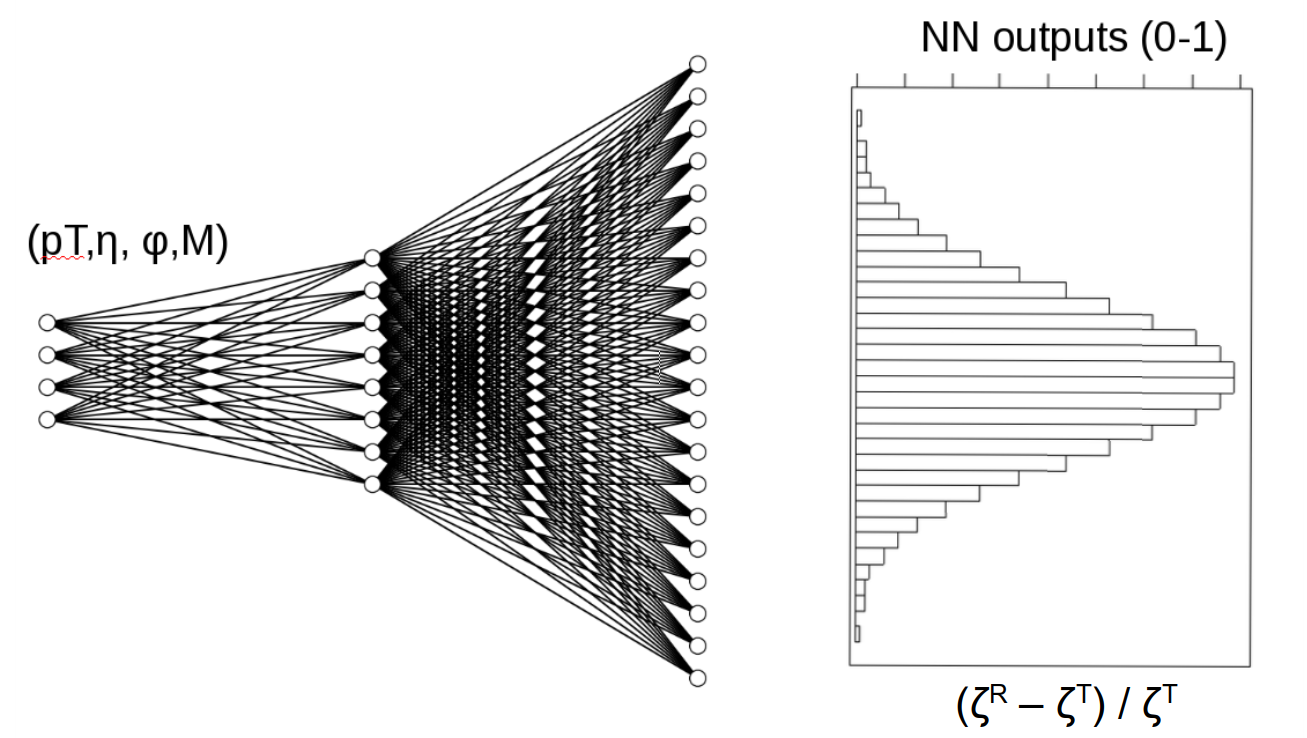
\includegraphics[width=0.8\textwidth]{figures/intro/nn_example.png}
  \caption{A schematic representation of the NN architecture for modelling the detector response to truth-level input variables.}
  \label{ann_example}
\end{figure}


%%%%%%%%%%%%%%%%%%%%%%%%%%%%%%%%%%%%%%%%%%%%% 
\section{Monte Carlo simulated event samples}
%%%%%%%%%%%%%%%%%%%%%%%%%%%%%%%%%%%%%%%%%%%%% 

Monte Carlo events used for this analysis were generated using the Madgraph generator~~\cite{Alwall:2014hca}. The simulated processes were a combination of $t\bar{t}$+jets and $\gamma$+jets {\color{red} What was the ratio}, which give a high rate of jets and lepton. 
Hadronic jets were reconstructed with the {\sc FastJet} package~\cite{Fastjet} using the anti-$k_T$ algorithm \cite{Cacciari:2008gp} with a distance parameter of 0.4. The detector simulation was performed with the Delphes package \cite{deFavereau:2013fsa} with an ATLAS-like detector geometry. 
The event samples used in this paper, before and after the fast simulation, are available from the HepSim database~\cite{Chekanov:2014fga}. In this paper only the transformation from truth-level jets to detector-level jets and only for \pt\ was performed, however the methodology should be object and parameter agnostic. Only truth jets which have been matched to a reconstructed Delphes jet are used. For the matching criteria the reconstructed jet that has the smallest $\Delta R=\sqrt{\Delta\phi^2+\Delta\eta^2}$, where $\Delta\phi=\phi^{\text{truth}}-\phi^{\text{reco}}$ and $\Delta\eta=\eta^{\text{truth}}-\eta^{\text{reco}}$, with respect to the truth jet is chosen. If this minimum $\Delta R$ is greater than 0.2, the truth-level jet is discarded.
The poor modeling of the NN below $\pt\sim 50$ GeV is due to the $\pt>15$ GeV requirement made on the reconstructed and truth jets. The requirement on the truth jets in combination with the width of the \ptRes, shown in Figure~\ref{fig:deltaTarget}, results in insufficient information being available to transform truth-level jet \pt s to reconstruction-level jet \pt s.
% Finally, only truth-reco jet pairs for which the truth jet has $\pt>60$ GeV are selected to move away from the $\pt>15$ GeV bound applied during the generation of the sample.
The final number of training jets used is two million while 500,000 jets were used as a testing sample.  

The distributions of quantities used as the input for the NN, \pt, $\eta$\, $\phi$, $m$, are shown in Figure~\ref{fig:nnInputsPrescaling}.

\begin{figure}[h]
  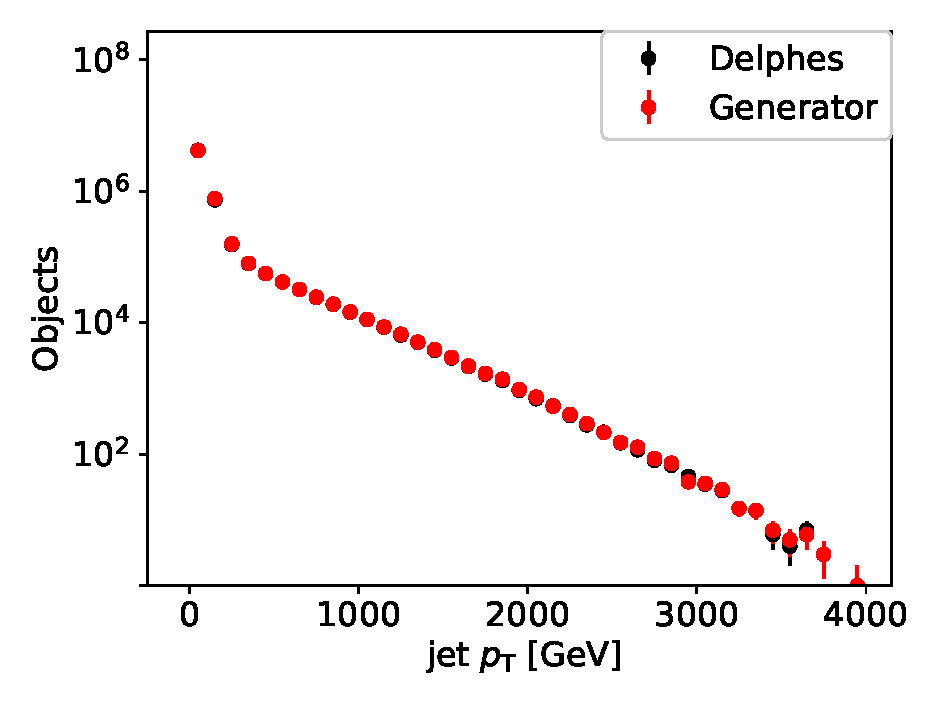
\includegraphics[width=0.48\textwidth]{figures/nn/jet_pT_prescaling_log.eps}
  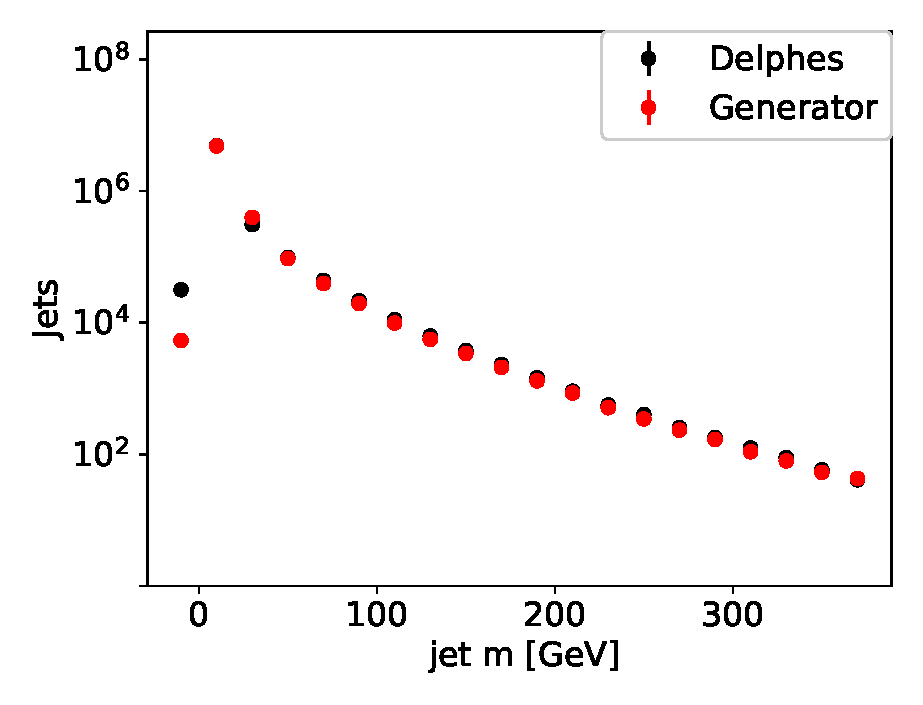
\includegraphics[width=0.48\textwidth]{figures/nn/jet_m_prescaling_log.eps}\\
  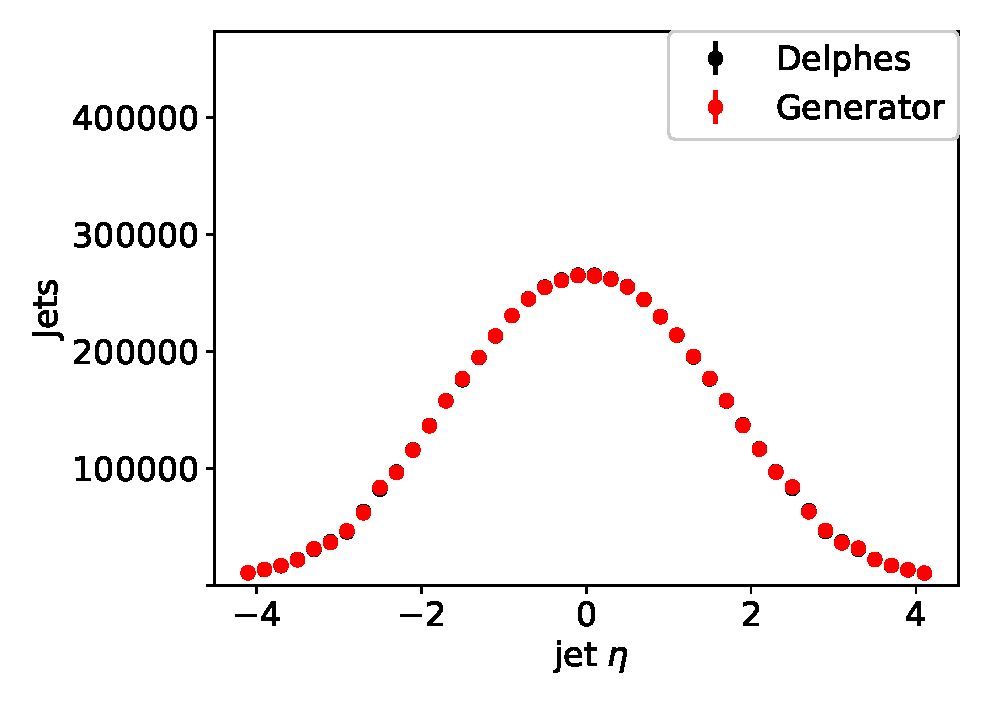
\includegraphics[width=0.48\textwidth]{figures/nn/jet_eta_prescaling.eps}
  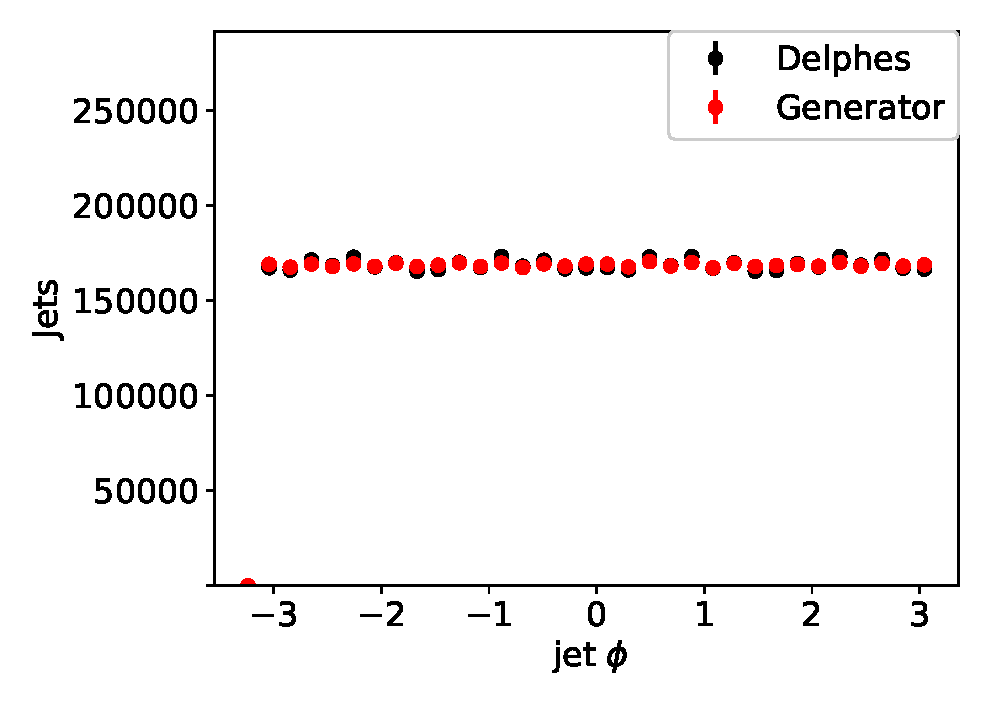
\includegraphics[width=0.48\textwidth]{figures/nn/jet_phi_prescaling.eps}
  \caption{Input variable shapes for truth-level (red) and detector-level quantities (black).}
  \label{fig:nnInputsPrescaling}
\end{figure}

To facilitate gradient descent in all direction of the input variables, the input variables are all scaled to be in the range [0,1]. This avoids the \pt\ and the mass from having a disproportional affect on the training of the NNs. The output variable, \ptRes, is also scaled to have values between 0 and 1. Only objects that 
are within the 1$^{\mathrm{st}}$ and 99$^{\mathrm{th}}$ percentile of the \ptRes\ distribution are considered in this study since objects outside this range are typically not used in physics analyses.

\begin{figure}[h]
  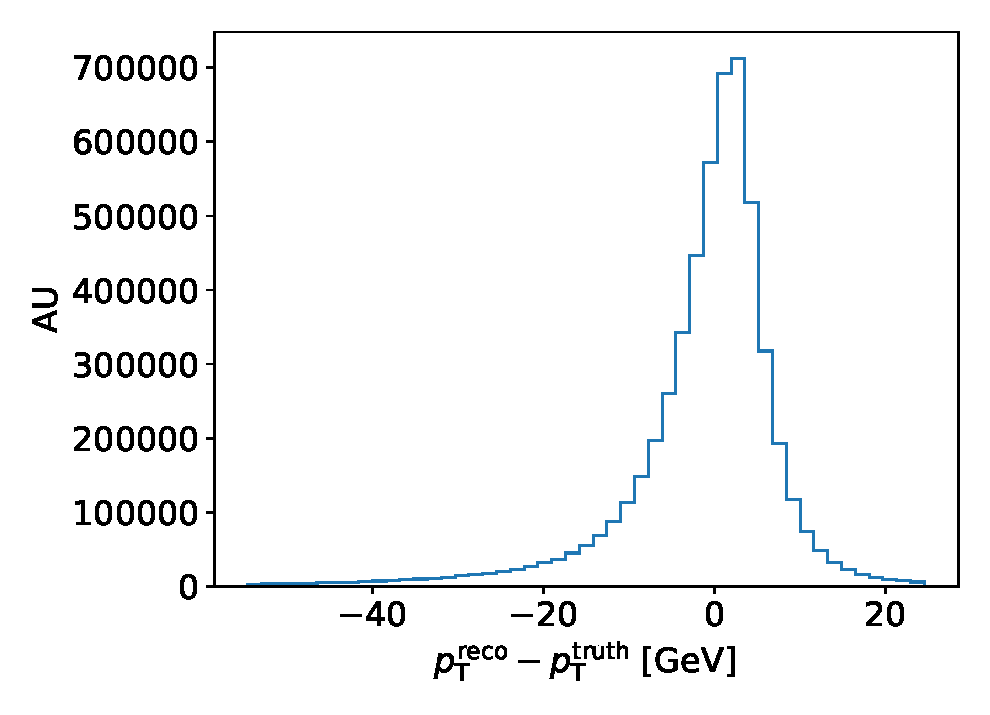
\includegraphics[width=0.6\textwidth]{figures/nn/pTRes_nobounds_prescaling.eps}
  \caption{Differences between truth-level and detector-level \pt.}
  \label{fig:deltaTarget}
\end{figure}

\section{Neural network structures}

An NN is trained with four input parameters, the scaled \pt, $\eta$, $\phi$, and $m$, and consist of five layers with 100 nodes each and with each node having a rectifier linear unit (ReLu) activation function. The output layer has 400 nodes with a softmax activation function. Finally, the NN is trained over 10 epochs with batch size 10 using the Adam~\cite{adam} optimizer with a learning rate of . The NN is implemented using Keras~\cite{chollet2015keras} with a tensorflow~\cite{tensorflow2015-whitepaper} backend.

%%%%%%%%%%%%%%%%%%%%%%%%%%%%%%%%%%%%%%%%%%%%% 
\section{Results}
%%%%%%%%%%%%%%%%%%%%%%%%%%%%%%%%%%%%%%%%%%%%%

After the NN has been trained to learn the pdf of \ptRes, the resulting learned pdf is compared to the Delphes pdf using the testing sample in Fig.~\ref{fig:pdfComp}. Good agreement is observed between the Delphes and NN pdfs, showing that the NN has learned the bulk distribution.

\begin{figure}[htb]
  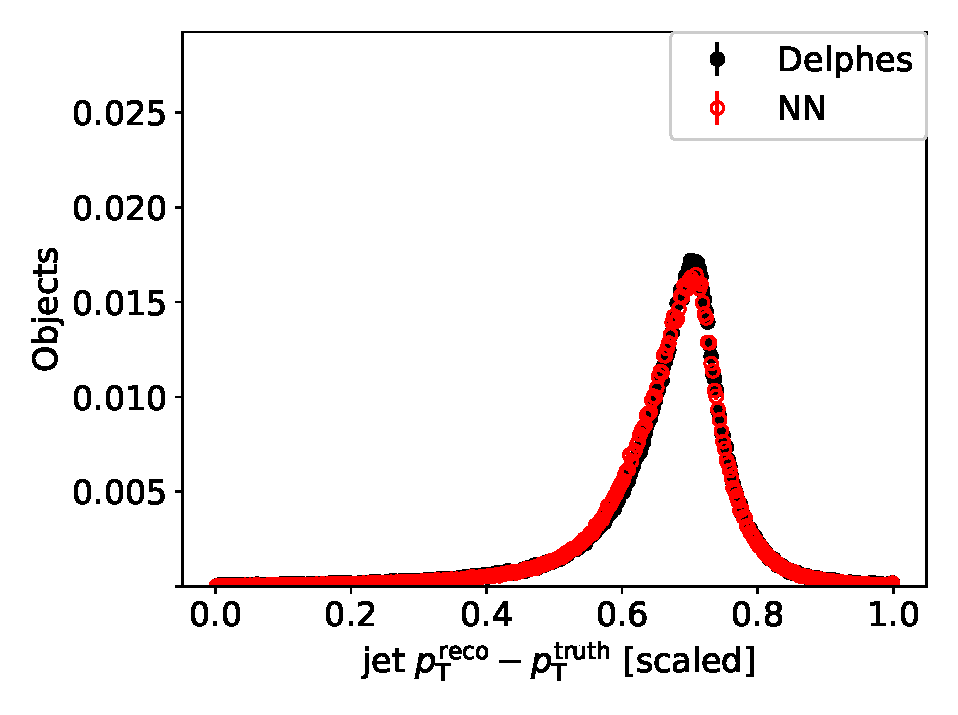
\includegraphics[width=0.48\textwidth]{figures/nn/jet_pTRes_batchSize10.eps}
  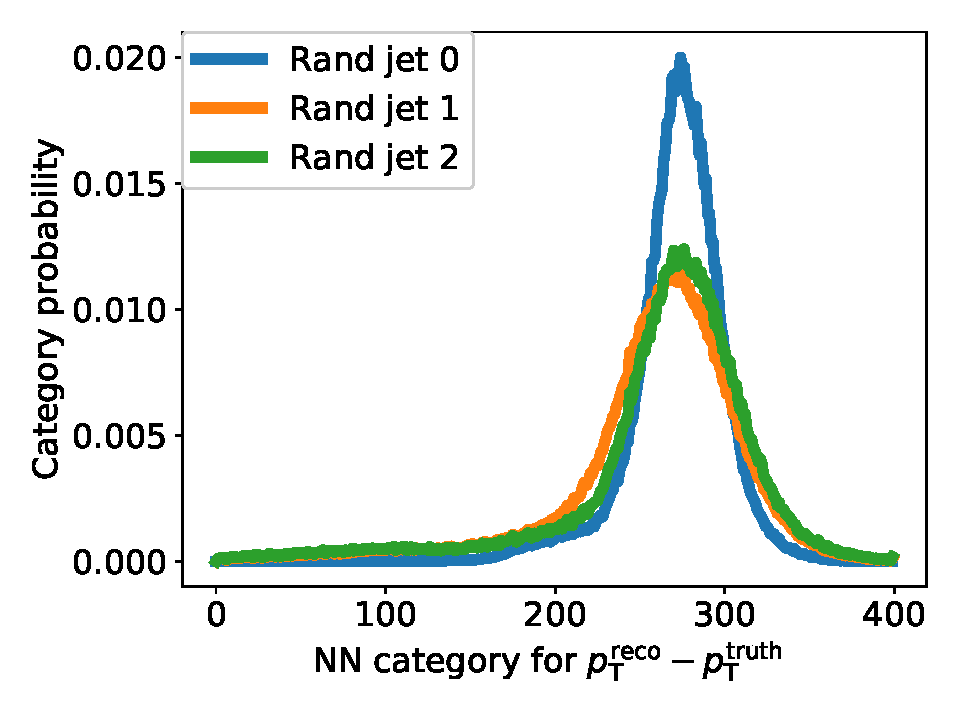
\includegraphics[width=0.48\textwidth]{figures/nn/nnOutput_pT_batchSize10.eps}
  \caption{Left: NN-generated jet \ptRes\ compared to detector-level jet \ptRes. Right: NN-generated jet pdfs for three randomly selected truth-level jets.}
  \label{fig:pdfComp}
\end{figure}

The NN predicts a pdf for each jet based on its input parameters (i.e. $\phi$, $\eta$, $m$). The pdfs for a set of randomly selected jets are shown in Fig.~\ref{fig:pdfComp}. These pdfs are then randomly sampled to produce a NN jet that mimic the detector-level jet. A comparison of the NN-generated and Delphes jet \pt for the testing sample is shown in Fig.~\ref{fig:nnVsDelphes}. The NN reproduces the jet \pt\ distribution of Delphes within 5\% for reconstructed jets with $\pt>50$ GeV. 

\begin{figure}[htb]
  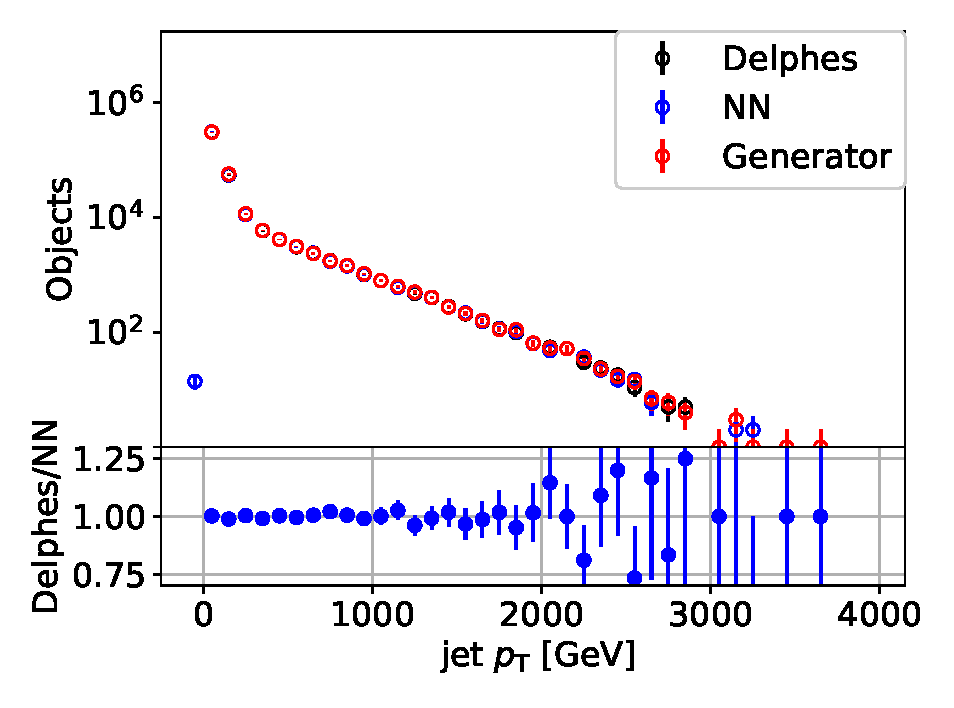
\includegraphics[width=0.6\textwidth]{figures/nn/jet_pT_genVsReco_origScale_test_batchSize10_log.eps}
  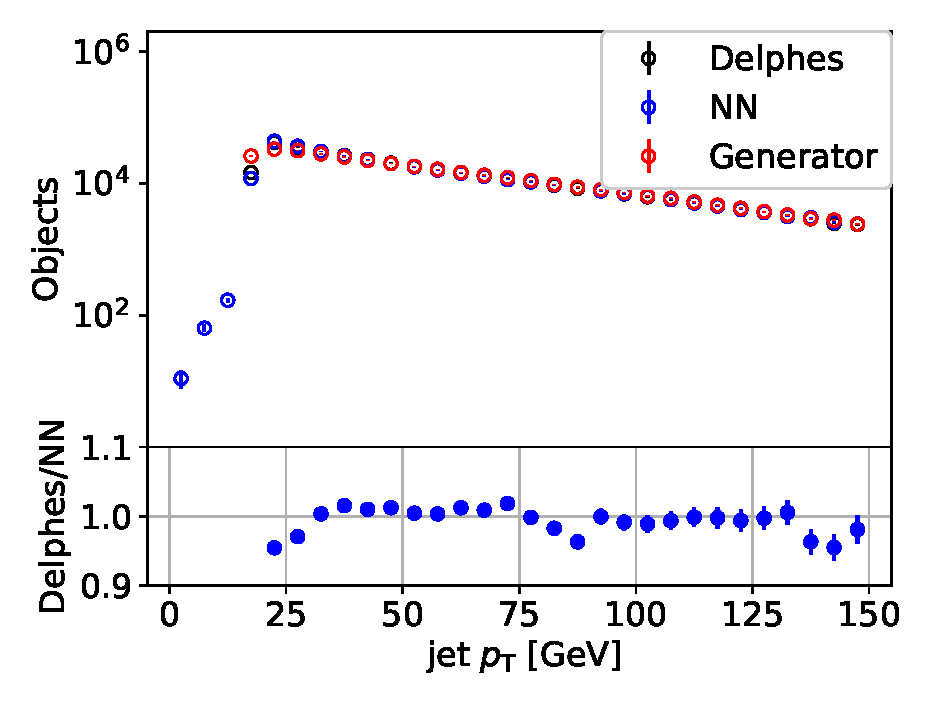
\includegraphics[width=0.6\textwidth]{figures/nn/jet_pT_genVsReco_origScale_zoom_test_batchSize10_log.eps}
  \caption{NN-generated jet \pt, mass, $\eta$, $\phi$ compared to truth-level and detector-level jet features. }
  \label{fig:nnVsDelphes}
\end{figure}

To test whether the NN learned correlations between input parameters and the \pt\ resolution, defined as $\frac{\ptRes}{\pt^{\text{truth}}}$, the jets were divided into central ($|\eta|<3.2$ and forward ($|\eta|>3.2$ jets), then the \pt\ resolution is compared between the two regions for both the Delphes jets as well as the NN-generated jets. These two regions in detectors have different calorimeter resolutions which results in different jet \pt\ resolutions and thus the \pt\ resolution is correlated with $|\eta|$. The resulting resolutions for both regions and for the training samples and jets are shown in Fig.~\ref{fig:nnRes}. The training sample was chosen because it has significantly more jets and due the low number of jets that have $|\eta|>3.2$, as can be seen in Fig.~\ref{fig:nnInputsPrescaling}. The NN reproduces the central jet resolution very well and doesn't perform as well in the forward region.

\begin{figure}[htb]
  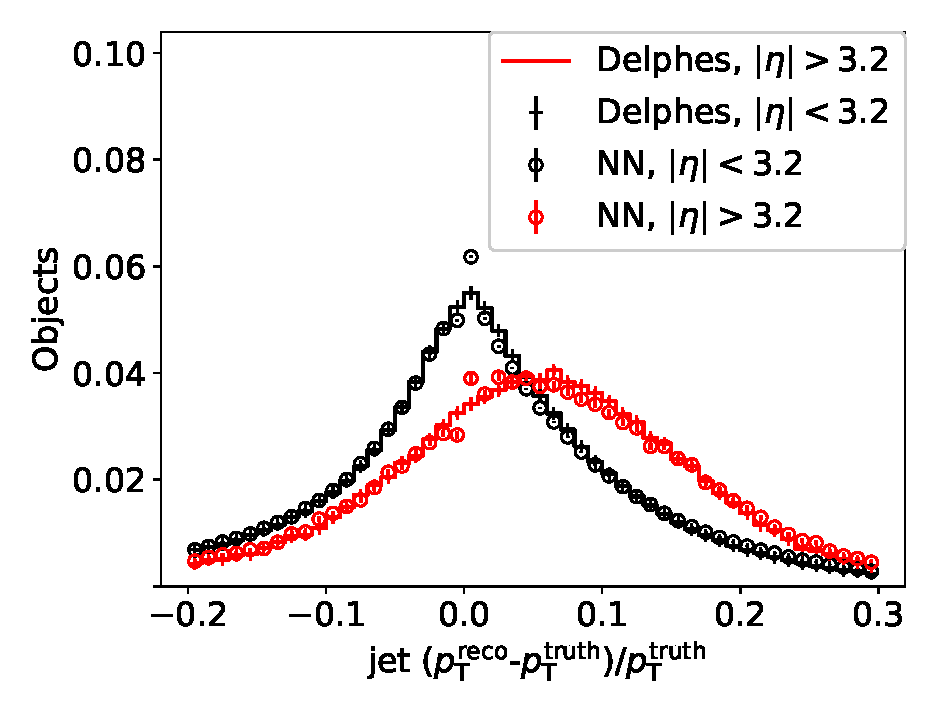
\includegraphics[width=0.6\textwidth]{figures/nn/jet_pTResEta_batchSize10.eps}
  \caption{Resolutions for the jet \pt\ for the training sample. }
  \label{fig:nnRes}
\end{figure}

\section{Hyperparameter scan}

% \section{Performance consideration?}
% For the binned NN, the training of one variable typically takes 30 min using 16 parallel processes.

\section{Conclusion}
We have shown that a truth-level quantity can be transformed to a reconstruction-level quantity using a multi-categorizing NN. 

\section*{Acknowledgments}
The submitted manuscript has been created by UChicago Argonne, LLC, Operator of Argonne National Laboratory (“Argonne”). Argonne, a U.S.  Department of Energy Office of Science laboratory, is operated under Contract No. DE-AC02-06CH11357. The U.S. Government retains for itself, 
and others acting on its behalf, a paid-up nonexclusive, irrevocable worldwide license in said article to reproduce, prepare derivative works, distribute copies to the public, and perform publicly and display publicly, by or on behalf of the Government.  The Department of Energy will provide public access to these results of federally sponsored research in accordance with the 
DOE Public Access Plan. \url{http://energy.gov/downloads/doe-public-access-plan}. Argonne National Laboratory’s work was funded by the U.S. Department of Energy, Office of High Energy Physics under contract DE-AC02-06CH11357. 



%%%%%%%%%%%%%%%%%%%%%% references %%%%%%%%%%%%%%%%%%%%%%%%%%%%%%
% \clearpage
\bibliographystyle{unsrt}   % this means that the order of references
			    % is dtermined by the order in which the
			    % \cite and \nocite commands appear
\bibliography{main}  % list here all the bibliographies that
			     % you need. 


\end{document}